% https://texample.net/tikz/examples/polar-coordinates-template/
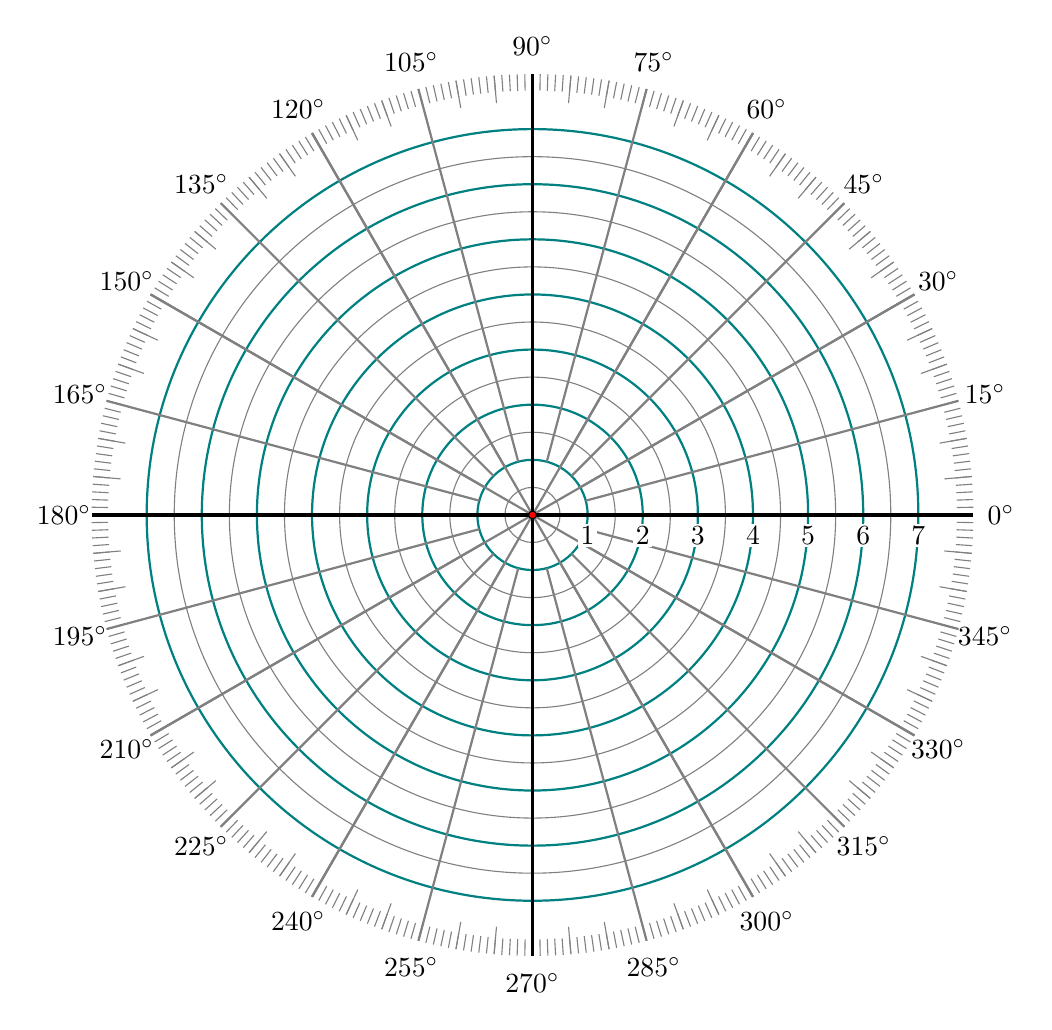
\begin{tikzpicture}[scale=.7]
    %Circles 
    \foreach \r in {1, 2,...,7}
        \draw[teal, thick] (0,0) circle (\r);    
    \foreach \r in {0.5, 1.5,...,7}
        \draw[gray, thin] (0,0) circle (\r);
    %1° Rays
    \foreach \a in {0, 1,...,359}
        \draw[gray] (\a:7.7) -- (\a:8);
    %5° Rays
    \foreach \a in {0, 5,...,359}
        \draw[gray] (\a:7.5) -- (\a:8);      
    %15° Rays
    \foreach \a in {0, 15,...,359}
        \draw[thick,gray] (\a:1) -- (\a:8); 
    %30° Rays
    \foreach \a in {0, 30,...,359}
        \draw[thick,gray] (0, 0) -- (\a:8);
    %Radius labels (background filled white)
    \foreach \r in {1, 2,...,7}
        \draw (\r,0) node[inner sep=1pt,below=3pt,rectangle,fill=white] {$\r$};
    %Main rays
    \foreach \a in {0, 90,...,359}
        \draw[very thick] (0, 0) -- (\a:8);
    %Angle labels  
    \foreach \a in {0, 15,...,359}
        \draw (\a: 8.5) node {$\a^\circ$};
    %Central point
    \draw[fill=red] (0,0) circle(0.7mm);
    \PolarPlot[0:2*pi][thick, orange]{t}
\end{tikzpicture}